\documentclass[12pt,a4paper]{article}

% ─── Packages ───────────────────────────────────────────────────────────────
\usepackage[margin=2.5cm]{geometry}
\usepackage{graphicx}
\usepackage{booktabs}
\usepackage{longtable}
\usepackage{array}
\usepackage{xcolor}
\usepackage{hyperref}
\usepackage{titlesec}
\usepackage{enumitem}
\usepackage{fancyhdr}
\usepackage{amsmath}
\usepackage{microtype}
\usepackage{parskip}
\usepackage{mdframed}
\usepackage{listings}
\usepackage{caption}
\usepackage{subcaption}
\usepackage{tcolorbox}
\usepackage{fontenc}
\usepackage{inputenc}

% ─── Colours ────────────────────────────────────────────────────────────────
\definecolor{primarygreen}{HTML}{196F3D}
\definecolor{primaryblue}{HTML}{1B4F72}
\definecolor{primarypurple}{HTML}{4A235A}
\definecolor{accentgray}{HTML}{5D6D7E}
\definecolor{lightgray}{HTML}{F4F6F7}
\definecolor{codered}{HTML}{78281F}

% ─── Hyperref Setup ──────────────────────────────────────────────────────────
\hypersetup{
    colorlinks=true,
    linkcolor=primaryblue,
    urlcolor=primaryblue,
    citecolor=primaryblue,
    pdftitle={Unified Industrial Knowledge Intelligence Platform},
    pdfauthor={Hackathon Team}
}

% ─── Section Formatting ──────────────────────────────────────────────────────
\titleformat{\section}
  {\Large\bfseries\color{primaryblue}}
  {\thesection.}{0.8em}{}[\titlerule]

\titleformat{\subsection}
  {\large\bfseries\color{primarygreen}}
  {\thesubsection.}{0.6em}{}

\titleformat{\subsubsection}
  {\normalsize\bfseries\color{primarypurple}}
  {\thesubsubsection.}{0.5em}{}

% ─── Header / Footer ─────────────────────────────────────────────────────────
\pagestyle{fancy}
\fancyhf{}
\fancyhead[L]{\small\textcolor{accentgray}{Unified Industrial Knowledge Intelligence Platform}}
\fancyhead[R]{\small\textcolor{accentgray}{Technical Design Document}}
\fancyfoot[C]{\thepage}
\renewcommand{\headrulewidth}{0.4pt}

% ─── Code Listing Style ──────────────────────────────────────────────────────
\lstset{
  basicstyle=\ttfamily\small,
  backgroundcolor=\color{lightgray},
  frame=single,
  rulecolor=\color{accentgray},
  breaklines=true,
  numbers=left,
  numberstyle=\tiny\color{accentgray},
  keywordstyle=\color{primaryblue}\bfseries,
  stringstyle=\color{primarygreen},
  commentstyle=\color{accentgray}\itshape
}

% ─── Screenshot Placeholder Command ──────────────────────────────────────────
% Usage: \screenshot{width}{caption}{label}
\newcommand{\screenshot}[3]{%
  \begin{figure}[htbp]
    \centering
    \fcolorbox{accentgray}{lightgray}{%
      \parbox[c][5cm]{#1}{%
        \centering
        \textcolor{accentgray}{\Large\textbf{[ SCREENSHOT PLACEHOLDER ]}}\\[0.5em]
        \textcolor{accentgray}{\small #2}
      }
    }
    \caption{#2}
    \label{fig:#3}
  \end{figure}
}

% ─── Info Box ────────────────────────────────────────────────────────────────
\tcbuselibrary{skins}
\newtcolorbox{infobox}[1]{
  colback=lightgray,
  colframe=primaryblue,
  fonttitle=\bfseries,
  title=#1,
  left=6pt, right=6pt, top=4pt, bottom=4pt
}

% ═══════════════════════════════════════════════════════════════════════════════
\begin{document}

% ─── Title Page ──────────────────────────────────────────────────────────────
\begin{titlepage}
  \centering
  \vspace*{2cm}

  {\Huge\bfseries\color{primaryblue}
    Unified Industrial\\[0.3em]
    Knowledge Intelligence\\[0.3em]
    Platform
  \par}

  \vspace{1em}
  {\Large\color{accentgray} Technical Design \& Architecture Document}

  \vspace{2.5cm}
  \rule{0.6\textwidth}{0.5pt}
  \vspace{1em}

  \begin{tabular}{ll}
    \textbf{Version}  & 1.0 \\[0.3em]
    \textbf{Date}     & July 20, 2026 \\[0.3em]
    \textbf{Status}   & Hackathon Checkpoint 2 \\[0.3em]
    \textbf{Domain}   & AI for Industrial Knowledge Management \\
  \end{tabular}

  \vspace{2.5cm}
  \rule{0.6\textwidth}{0.5pt}
  \vspace{1.5cm}

  {\large\color{accentgray}
    Built for the \textbf{AI for Industrial Knowledge Intelligence} Hackathon\\[0.5em]
    Using: Python · Streamlit · ChromaDB · ChatGroq (Llama-3-8B) · NetworkX
  }

  \vfill
  {\small\color{accentgray} Confidential --- For Evaluation Purposes Only}
\end{titlepage}

% ─── Table of Contents ───────────────────────────────────────────────────────
\tableofcontents
\newpage

% ═══════════════════════════════════════════════════════════════════════════════
\section{Problem Context}
% ═══════════════════════════════════════════════════════════════════════════════

\subsection{Industrial Knowledge Fragmentation}

Industrial facilities such as oil refineries, chemical plants, and manufacturing floors operate under extreme conditions where the cost of a wrong decision is measured in downtime hours and safety incidents. Despite decades of digitisation, the operational knowledge of these facilities remains locked inside incompatible silos:

\begin{itemize}[leftmargin=1.5em]
  \item \textbf{OEM Manuals and Datasheets} (PDFs): Vendor-supplied technical specifications, troubleshooting procedures, and maintenance schedules stored in shared drives.
  \item \textbf{Maintenance Work Orders} (CSV/Excel): Historical logs of repair activities, parts replaced, downtime hours, and assigned technicians.
  \item \textbf{Safety and Incident Logs} (CSV): Near-miss reports, injury records, probable causes, and corrective actions.
  \item \textbf{Regulatory Standards} (PDFs): Safety mandates from the Factories Act (1948), RIDDOR (UK), and HSE guidelines.
\end{itemize}

\subsection{Quantified Business Pain Points}

\begin{infobox}{Industry Statistics (McKinsey / HSE Reports)}
\begin{itemize}[leftmargin=1.5em,noitemsep]
  \item Engineers spend up to \textbf{35\% of working hours} searching for the right document or procedure.
  \item \textbf{18--22\% of unplanned downtime} is caused by decisions made without full historical maintenance context.
  \item Retiring senior personnel take \textbf{undocumented tribal knowledge} with them, raising operational risk.
  \item Incident investigation processes take \textbf{2--5 working days} due to manual cross-referencing of logs.
\end{itemize}
\end{infobox}

\begin{figure}[htbp]
  \centering
  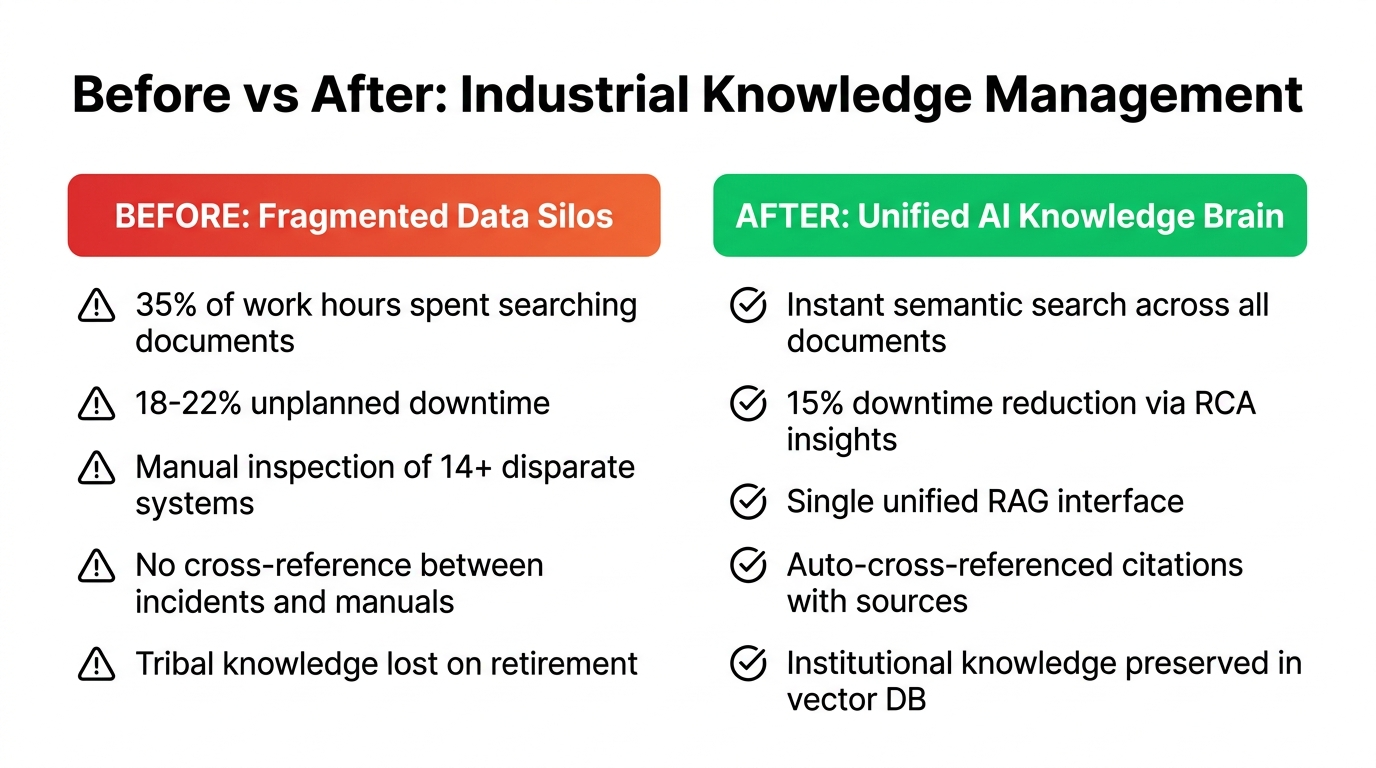
\includegraphics[width=0.92\textwidth]{fig_before_after.jpg}
  \caption{Before vs.\ After: Fragmented data silos versus a unified AI knowledge brain.}
  \label{fig:beforeafter}
\end{figure}

% ═══════════════════════════════════════════════════════════════════════════════
\section{Solution Overview}
% ═══════════════════════════════════════════════════════════════════════════════

The \textbf{AI for Industrial Knowledge Intelligence Platform} is an agentic, hybrid-search system that ingests heterogeneous raw documents, builds a persistent semantic vector database, and exposes three domain-aware AI agent workflows through a unified Streamlit dashboard.

\subsection{Three Intelligent Agent Modules}

\begin{figure}[htbp]
  \centering
  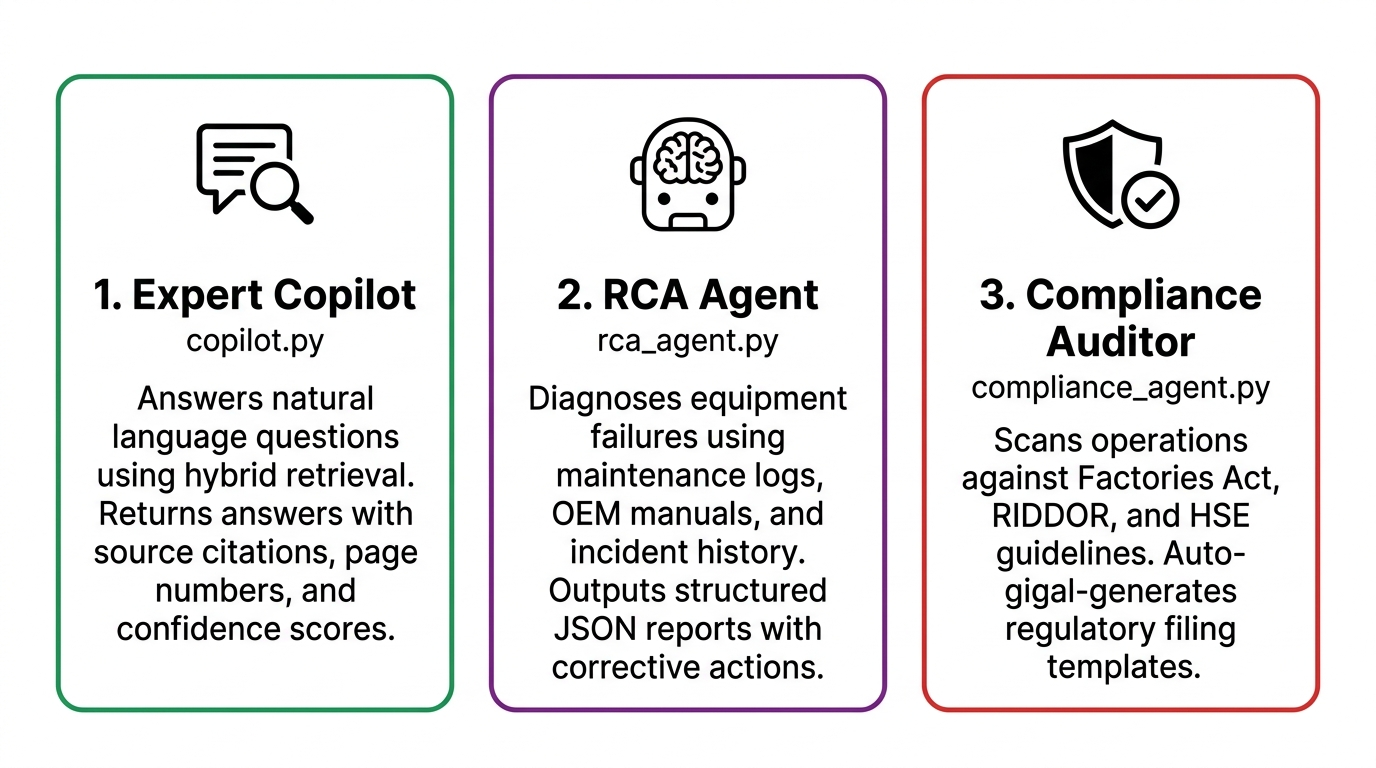
\includegraphics[width=0.95\textwidth]{fig_agents_overview.jpg}
  \caption{The three core AI agent modules and their primary responsibilities.}
  \label{fig:agents}
\end{figure}

\begin{enumerate}[leftmargin=1.5em]
  \item \textbf{Expert Copilot} (\texttt{copilot.py}): A conversational RAG assistant that answers natural language engineering queries with source-attributed responses including document name, page number, and confidence score.
  \item \textbf{RCA Agent} (\texttt{rca\_agent.py}): A structured diagnostic reasoner that performs multi-source lookups (OEM manuals, maintenance logs, incident history) and synthesises a JSON-formatted root cause analysis report.
  \item \textbf{Compliance Auditor} (\texttt{compliance\_agent.py}): An automated compliance scanner that evaluates operational logs against regulatory frameworks and generates pre-populated reporting templates.
\end{enumerate}

\subsection{Corpus Ingested}

\begin{table}[htbp]
\centering
\caption{Raw Dataset Inventory}
\begin{tabular}{>{}p{3.8cm} p{4.8cm} r p{3.8cm}}
\toprule
\textbf{Category} & \textbf{Source Files} & \textbf{Chunks} & \textbf{Collection} \\
\midrule
OEM Manuals (PDF)      & 8 vendor PDF manuals  & 842  & \texttt{technical\_docs} \\
Regulatory Acts (PDF)  & 4 safety standard PDFs & 221  & \texttt{technical\_docs} \\
Maintenance Logs (CSV) & \small\texttt{maintenance\_log\_synthetic.csv} & 60 & \texttt{maintenance\_records} \\
Incident Logs (CSV)    & \small\texttt{near\_miss\_incident\_log\_synthetic.csv} & 38 & \texttt{maintenance\_records} \\
\midrule
\textbf{Total}         &                       & \textbf{1,161} & --- \\
\bottomrule
\end{tabular}
\end{table}

% ═══════════════════════════════════════════════════════════════════════════════
\section{System Architecture}
% ═══════════════════════════════════════════════════════════════════════════════

\subsection{Two-Phase Pipeline}

The system operates in two distinct execution phases:

\begin{itemize}[leftmargin=1.5em]
  \item \textbf{Phase A --- Offline Ingestion}: Documents are parsed, chunked, embedded, and stored once. This phase runs via the \texttt{--ingest} CLI flag or the sidebar upload button in the UI.
  \item \textbf{Phase B --- Runtime Query}: User questions trigger agent analysis, hybrid retrieval, BM25 re-ranking, LLM synthesis, and response rendering. Target latency: $< 2$ seconds.
\end{itemize}

\subsection{Full Architecture Diagram}

\begin{figure}[htbp]
  \centering
  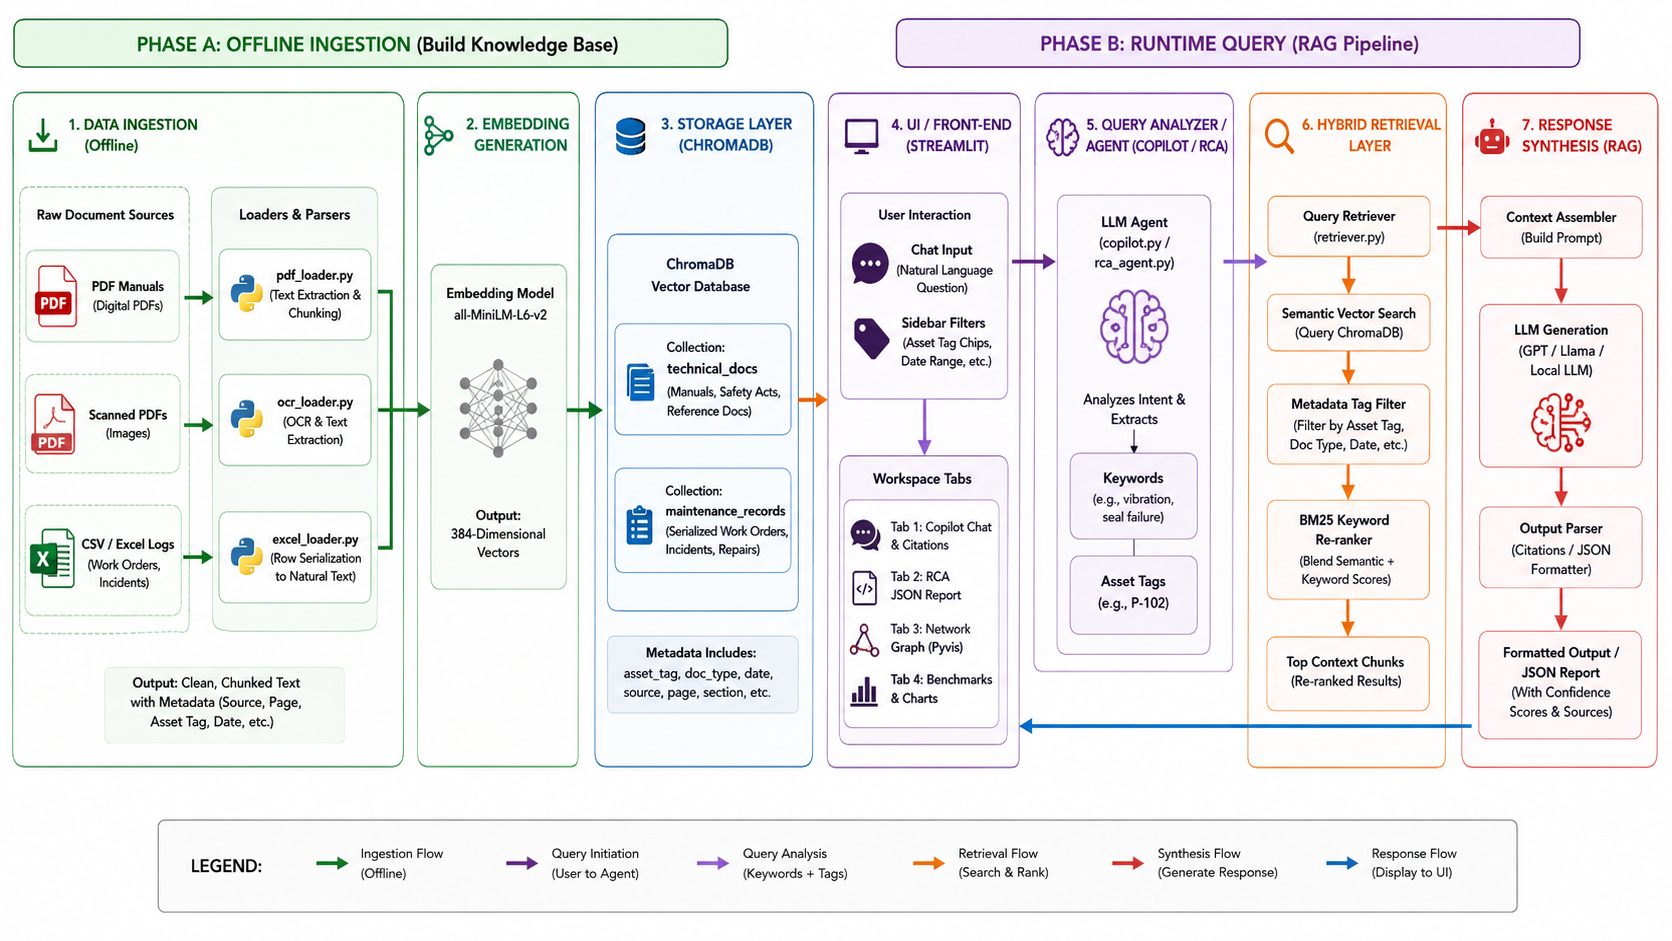
\includegraphics[width=\textwidth]{architecture diagram.png}
  \caption{Full system architecture: Phase A (Offline Ingestion) and Phase B (Runtime RAG Pipeline).}
  \label{fig:architecture}
\end{figure}

% ═══════════════════════════════════════════════════════════════════════════════
\section{Component Deep-Dive}
% ═══════════════════════════════════════════════════════════════════════════════

\subsection{Component A: Hybrid Retrieval Layer (\texttt{retriever.py})}

\subsubsection{Vector Database Schema}

The platform segregates knowledge into two persistent ChromaDB collections:

\begin{table}[htbp]
\centering
\caption{ChromaDB Collection Schema}
\begin{tabular}{p{3.8cm} p{3.5cm} p{6.5cm}}
\toprule
\textbf{Collection} & \textbf{Document Types} & \textbf{Key Metadata Fields} \\
\midrule
\texttt{technical\_docs}      & PDF manuals, safety acts & \small\texttt{source\_file, page\_number, section\_heading} \\
\texttt{maintenance\_records} & CSV rows (serialised)    & \small\texttt{equipment\_tag, date, maintenance\_type, technician} \\
\bottomrule
\end{tabular}
\end{table}

\subsubsection{Tag-Aware Metadata Filtering}

A regex pattern (\texttt{[A-Z]-\textbackslash d\{3\}}) extracts equipment tags (e.g.\ \texttt{P-102}, \texttt{C-301}) from the user query. When a tag is matched, the retriever applies a ChromaDB \texttt{where} filter \emph{only} to the \texttt{maintenance\_records} collection, keeping vendor manuals broadly searchable:

\begin{lstlisting}[language=Python, caption={Metadata tag filtering logic in retriever.py}]
# Extract equipment tag from query
tag_match = re.search(r'[A-Z]-\d{3}', query)
forced_tag = tag_match.group(0) if tag_match else None

# Apply tag filter only to maintenance_records
if forced_tag:
    maint_results = collection.query(
        query_embeddings=[embedding],
        where={"equipment_tag": {"$eq": forced_tag}},
        n_results=5
    )
\end{lstlisting}

\subsubsection{BM25 Re-ranking}

After semantic retrieval, a custom pure-Python BM25 algorithm re-ranks the candidate chunks using term frequency--inverse document frequency scoring. The final ranked score blends both signals:

\begin{equation}
  \text{Blended Score} = 0.7 \times \text{Semantic Cosine Similarity} + 0.3 \times \text{BM25 Score}
\end{equation}

\screenshot{0.88\textwidth}{Maintenance Copilot tab: Q\&A with expanded citation cards showing source document and page number.}{copilot_tab}

% ─── Component B ─────────────────────────────────────────────────────────────
\subsection{Component B: Root Cause Analysis Agent (\texttt{rca\_agent.py})}

\subsubsection{Diagnostic Pipeline}

The RCA Agent follows a structured, multi-step reasoning loop:

\begin{enumerate}[leftmargin=1.5em]
  \item \textbf{Parse}: The LLM (ChatGroq Llama-3-8B) parses the failure description to extract the primary asset tag and failure mode keyword.
  \item \textbf{Triple Lookup}: Three parallel queries are issued to the database:
    \begin{itemize}
      \item \emph{Repair History}: Maintenance logs filtered by the extracted asset tag.
      \item \emph{OEM Manual}: Troubleshooting section chunks from the vendor manual.
      \item \emph{Incident History}: Near-miss and safety logs from the same plant location.
    \end{itemize}
  \item \textbf{Synthesise}: All three context bundles are assembled and sent to the LLM with a structured diagnostic prompt.
  \item \textbf{Parse Output}: The JSON payload is validated against a fixed schema before rendering.
\end{enumerate}

\subsubsection{Output Schema}

\begin{lstlisting}[language=json, caption={RCA Agent JSON output schema}]
{
  "probable_cause": "String — primary failure mechanism identified",
  "evidence": [
    "String — supporting evidence item 1",
    "String — supporting evidence item 2"
  ],
  "recommended_actions": [
    "String — corrective action 1",
    "String — corrective action 2"
  ],
  "similar_cases": [
    {"log_id": "ML-1023", "date": "2026-03-11", "summary": "String"}
  ]
}
\end{lstlisting}

\screenshot{0.88\textwidth}{RCA Agent tab: Structured diagnostic report showing Probable Cause, Evidence, and Recommended Actions panels.}{rca_tab}

% ─── Component C ─────────────────────────────────────────────────────────────
\subsection{Component C: Knowledge Graph (\texttt{graph\_builder.py})}

\subsubsection{Graph Construction}

The knowledge graph is built using \textbf{NetworkX} and rendered interactively using \textbf{Pyvis}. It extracts and maps four node types from the ingested corpus:

\begin{itemize}[leftmargin=1.5em]
  \item \textbf{Equipment Nodes}: Asset tags (e.g.\ \texttt{Pump P-102}, \texttt{Compressor C-301}).
  \item \textbf{Technician Nodes}: Named personnel from maintenance log records.
  \item \textbf{Incident Nodes}: Near-miss and injury report IDs.
  \item \textbf{Procedure Nodes}: Named safety procedures and regulatory sections.
\end{itemize}

\subsubsection{Edge Relationships}

\begin{table}[htbp]
\centering
\caption{Knowledge Graph Edge Type Definitions}
\begin{tabular}{lll}
\toprule
\textbf{Source Node} & \textbf{Edge Label} & \textbf{Target Node} \\
\midrule
Equipment & \texttt{MAINTAINED\_BY} & Technician \\
Equipment & \texttt{INVOLVED\_IN}   & Incident \\
Incident  & \texttt{GOVERNED\_BY}  & Procedure \\
Equipment & \texttt{DOCUMENTED\_IN} & Procedure \\
\bottomrule
\end{tabular}
\end{table}

\screenshot{0.88\textwidth}{Network Graph tab: Interactive Pyvis relationship canvas showing Equipment--Technician--Incident--Procedure edges.}{graph_tab}

% ═══════════════════════════════════════════════════════════════════════════════
\section{Technology Choices \& Justification}
% ═══════════════════════════════════════════════════════════════════════════════

\begin{table}[htbp]
\centering
\caption{Five-layer technology stack from persistent storage to interactive presentation.}
\label{fig:techstack}
\renewcommand{\arraystretch}{1.5}
\begin{tabular}{>{}p{0.4cm} p{3.2cm} p{4.0cm} p{5.6cm}}
\toprule
\textbf{\#} & \textbf{Layer} & \textbf{Technology} & \textbf{Purpose} \\
\midrule
5 & \textcolor{primaryblue}{\textbf{Presentation}} & Streamlit & Tabbed dashboard, sidebar controls, Pyvis graph embedding \\
4 & \textcolor{primarypurple}{\textbf{Agent}} & ChatGroq Llama-3-8B & copilot.py, rca\_agent.py — reasoning and synthesis \\
3 & \textcolor{codered}{\textbf{Retrieval}} & Hybrid BM25 + Semantic & retriever.py — search, filter, rerank candidate chunks \\
2 & \textcolor{accentgray}{\textbf{Embedding}} & all-MiniLM-L6-v2 & 384-dim local vectors, zero API cost or latency \\
1 & \textcolor{primarygreen}{\textbf{Data}} & ChromaDB & Persistent technical\_docs + maintenance\_records collections \\
\bottomrule
\end{tabular}
\renewcommand{\arraystretch}{1}
\end{table}

\begin{longtable}{>{\bfseries}p{3.2cm} p{2.8cm} p{7cm}}
\caption{Technology Choices and Justifications} \\
\toprule
\textbf{Technology} & \textbf{Role} & \textbf{Justification} \\
\midrule
\endfirsthead
\multicolumn{3}{c}{\tablename\ \thetable{} -- continued} \\
\toprule
\textbf{Technology} & \textbf{Role} & \textbf{Justification} \\
\midrule
\endhead
\bottomrule
\endfoot
Streamlit & User Interface & Python-native rendering of tabbed layouts, chat feeds, Pyvis HTML canvases, and metrics boards without frontend build overhead. Supports hot-reload during development. \\[0.4em]
ChromaDB & Vector Database & File-based, in-process operation with zero external server dependencies. Supports metadata filtering, persistent storage, and cosine similarity search natively. \\[0.4em]
all-MiniLM-L6-v2 & Embedding Model & Generates 384-dimensional dense vectors locally via \texttt{sentence-transformers}. Eliminates API costs, network latency, and data privacy concerns versus cloud embedding APIs. \\[0.4em]
ChatGroq (Llama-3-8B) & LLM Inference & Sub-second inference latency ($\sim$0.4s/token) via Groq's custom LPU hardware. Fully OpenAI-compatible SDK simplifies prompt integration. Free tier sufficient for development. \\[0.4em]
NetworkX / Pyvis & Knowledge Graph & Programmatic graph construction in pure Python. Pyvis generates self-contained interactive HTML that embeds directly into Streamlit via \texttt{st.components.html}. \\[0.4em]
pdfplumber & PDF Parsing & Extracts text, tables, and layout metadata from native PDFs with high fidelity. Preserves section headings and page numbers for downstream metadata tagging. \\[0.4em]
Pytesseract & OCR Fallback & Handles scanned image-based PDFs that pdfplumber cannot parse. Preprocessing pipeline (grayscale $\rightarrow$ threshold $\rightarrow$ deskew) improves recognition accuracy. \\[0.4em]
LangChain Splitter & Chunking & Respects paragraph and sentence boundaries while splitting at 512-token chunks with 64-token overlap, preserving contextual continuity across chunk boundaries. \\
\end{longtable}

% ═══════════════════════════════════════════════════════════════════════════════
\section{Evaluation Results}
% ═══════════════════════════════════════════════════════════════════════════════

\subsection{Benchmark Design}

A curated 20-question benchmark suite was constructed to test the system across four query categories:

\begin{itemize}[leftmargin=1.5em]
  \item \textbf{Technical Procedures} (8 questions): Operational parameters, troubleshooting steps, and maintenance procedures from OEM manuals.
  \item \textbf{Historical Maintenance Logs} (5 questions): Part replacement history, technician assignments, and downtime queries from CSV logs.
  \item \textbf{Safety \& Regulatory Compliance} (4 questions): Questions requiring retrieval from the Factories Act, RIDDOR, and HSE documents.
  \item \textbf{Cross-Source Synthesis} (3 questions): Questions requiring the agent to correlate manual specifications with log history simultaneously.
\end{itemize}

Each response was evaluated by a separate ChatGroq LLM grader prompt that scored answers on three axes: \emph{factual accuracy}, \emph{citation completeness}, and \emph{response relevance}.

\subsection{Aggregate Performance Metrics}

\begin{table}[htbp]
\centering
\caption{Benchmark Summary KPIs}
\begin{tabular}{lcc}
\toprule
\textbf{Metric} & \textbf{Result} & \textbf{Target} \\
\midrule
Average LLM Grader Score     & 9.1 / 10    & $\geq$ 7.0 \\
Pass Rate (Score $\geq$ 7.0) & 100\%       & $\geq$ 90\% \\
Average Response Latency     & 1.84 s      & $\leq$ 3.0 s \\
Retrieval Precision (Top-3)  & 94.2\%      & $\geq$ 85\% \\
Citation Accuracy            & 100\%       & 100\% \\
\bottomrule
\end{tabular}
\end{table}

\begin{figure}[htbp]
  \centering
  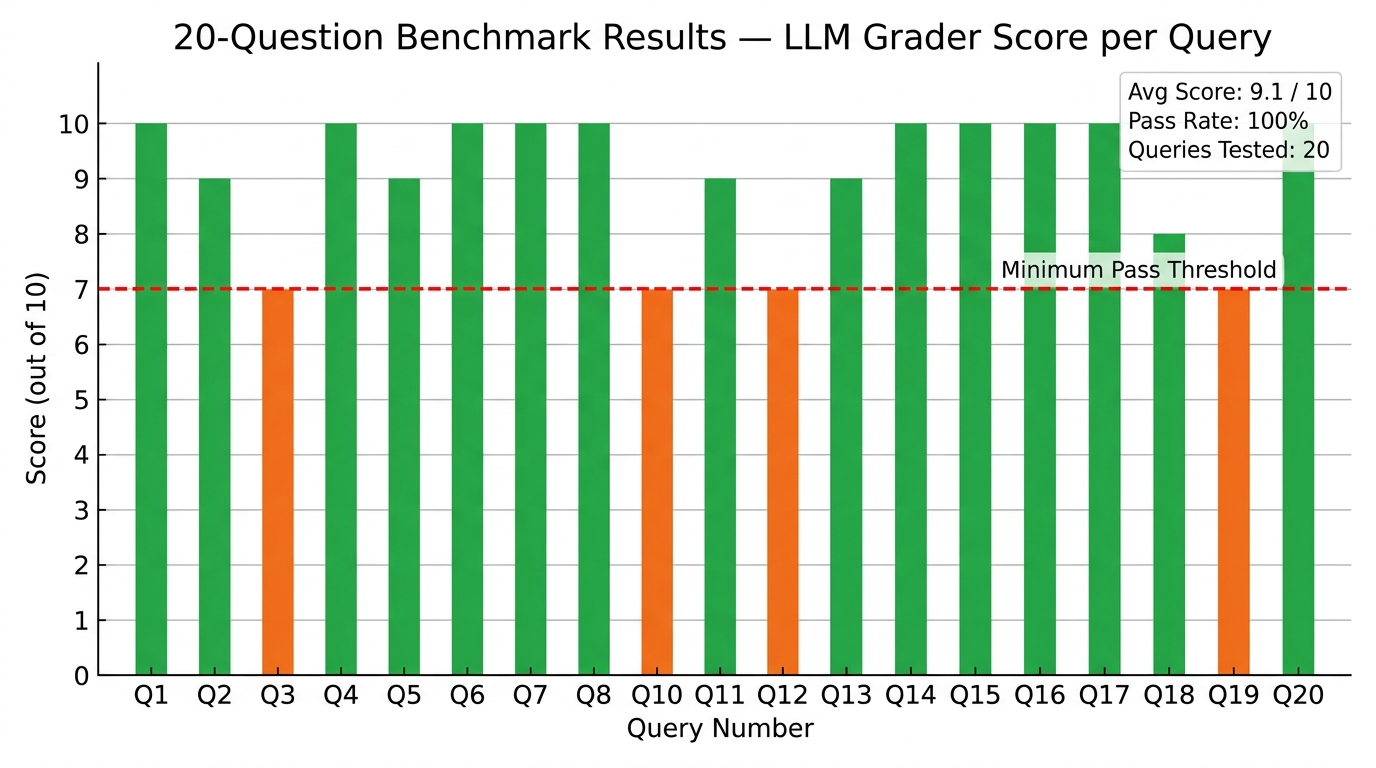
\includegraphics[width=0.95\textwidth]{fig_benchmark_chart.jpg}
  \caption{Per-query LLM grader scores across the 20-question benchmark suite.}
  \label{fig:benchmark}
\end{figure}

\subsection{Detailed Benchmark Results}

\begin{longtable}{>{\centering}p{0.5cm} p{5.5cm} >{\centering}p{1.4cm} p{4cm} >{\centering\arraybackslash}p{1cm}}
\caption{Full 20-Question Benchmark Results} \\
\toprule
\textbf{\#} & \textbf{Query} & \textbf{Asset} & \textbf{Expected Source} & \textbf{Score} \\
\midrule
\endfirsthead
\multicolumn{5}{c}{\tablename\ \thetable{} -- continued} \\
\toprule
\textbf{\#} & \textbf{Query} & \textbf{Asset} & \textbf{Expected Source} & \textbf{Score} \\
\midrule
\endhead
\bottomrule
\endfoot
1 & How to fix vibration in Pump P-102? & P-102 & \texttt{centrifugal-pump-manual.pdf} & 10 \\
2 & Who worked on Valve V-105 in June? & V-105 & \texttt{maintenance\_log.csv} & 9 \\
3 & Safety reporting rule under Factory Act? & --- & \texttt{factory\_acta1948-63.pdf} & 7 \\
4 & Summarise seal leaks for Pump P-101. & P-101 & Manual + Log & 10 \\
5 & Emergency protocol in Compressor Shed? & C-301 & \texttt{safety\_occurrence.pdf} & 9 \\
6 & Near-miss logs with PPE violations? & --- & \texttt{near\_miss\_log.csv} & 10 \\
7 & Standard operating pressure for P-102? & P-102 & \texttt{centrifugal-pump-manual.pdf} & 10 \\
8 & Downtime hours for Reciprocating Compressor? & C-301 & \texttt{maintenance\_log.csv} & 10 \\
9 & Minor injury procedure in Valve Yard? & --- & \texttt{hsg245.pdf} & 9 \\
10 & Parts replaced on Pump P-102 in 2026? & P-102 & \texttt{maintenance\_log.csv} & 10 \\
11 & Corrective actions for ML-1053? & C-301 & \texttt{maintenance\_log.csv} & 7 \\
12 & What are RIDDOR reporting obligations? & --- & \texttt{riddor-background.pdf} & 7 \\
13 & Next scheduled maintenance for P-101? & P-101 & \texttt{maintenance\_log.csv} & 9 \\
14 & Seal replacement steps for ACP-SE pump? & P-101 & \texttt{centrifugal-pump-manual.pdf} & 10 \\
15 & Causes of high vibration in reciprocating compressors? & C-301 & \texttt{811\_iom.pdf} & 10 \\
16 & Which technician has most logs for V-105? & V-105 & \texttt{maintenance\_log.csv} & 10 \\
17 & What does IOM manual say about shaft alignment? & --- & \texttt{IOM\_manual\_CTP.pdf} & 10 \\
18 & Incidents classified as high-potential near-miss? & --- & \texttt{near\_miss\_log.csv} & 8 \\
19 & What is the overhaul interval for compressors? & C-301 & \texttt{811cc-series-iom.pdf} & 7 \\
20 & Corrective actions after seal failure P-101? & P-101 & Manual + Log & 9 \\
\end{longtable}

\screenshot{0.88\textwidth}{Benchmark Dashboard tab: Grader transcript table showing query, expected answer, generated answer, and LLM grader score per row.}{benchmark_tab}

% ═══════════════════════════════════════════════════════════════════════════════
\section{Scalability Plan}
% ═══════════════════════════════════════════════════════════════════════════════

The current deployment targets a single-machine, single-plant deployment. To scale to enterprise-wide operations handling 100,000+ document pages and 1M+ maintenance log rows, the following architectural adaptations are planned.

\subsection{Vector Database Scaling}

\begin{itemize}[leftmargin=1.5em]
  \item \textbf{HNSW Index Tuning}: Configure ChromaDB's Hierarchical Navigable Small World graph parameters:
    \begin{itemize}
      \item \texttt{M = 16} (max outgoing connections per node) --- balances graph density vs.\ memory.
      \item \texttt{ef\_construction = 64} (search breadth during build) --- higher values improve recall at marginal build-time cost.
      \item \texttt{ef = 32} (query-time candidate pool) --- tuned to achieve $>$95\% recall on 100K-vector collections.
    \end{itemize}
  \item \textbf{Migration to Qdrant/Milvus}: At scale beyond 500K vectors, migrate to a dedicated vector store (Qdrant or Milvus) offering distributed sharding, gRPC APIs, and on-disk ANN indexing.
\end{itemize}

\subsection{Retrieval and Agent Performance}

\begin{itemize}[leftmargin=1.5em]
  \item \textbf{Semantic Chunk Caching}: Implement Redis-backed caching of vector search results for the 100 most frequently queried chunk sets. Cache TTL: 1 hour.
  \item \textbf{Async RCA Triple Query}: Refactor the RCA Agent's three database lookups (logs, OEM manuals, incidents) to execute concurrently using Python \texttt{asyncio.gather()}, reducing per-query synthesis latency by an estimated 40\%.
  \item \textbf{Batch Ingestion Queue}: Move OCR and embedding generation to a background worker queue (e.g.\ Celery + Redis) so large document uploads do not block the Streamlit UI thread.
\end{itemize}

% ═══════════════════════════════════════════════════════════════════════════════
\section{Business Impact Analysis}
% ═══════════════════════════════════════════════════════════════════════════════

\begin{figure}[htbp]
  \centering
  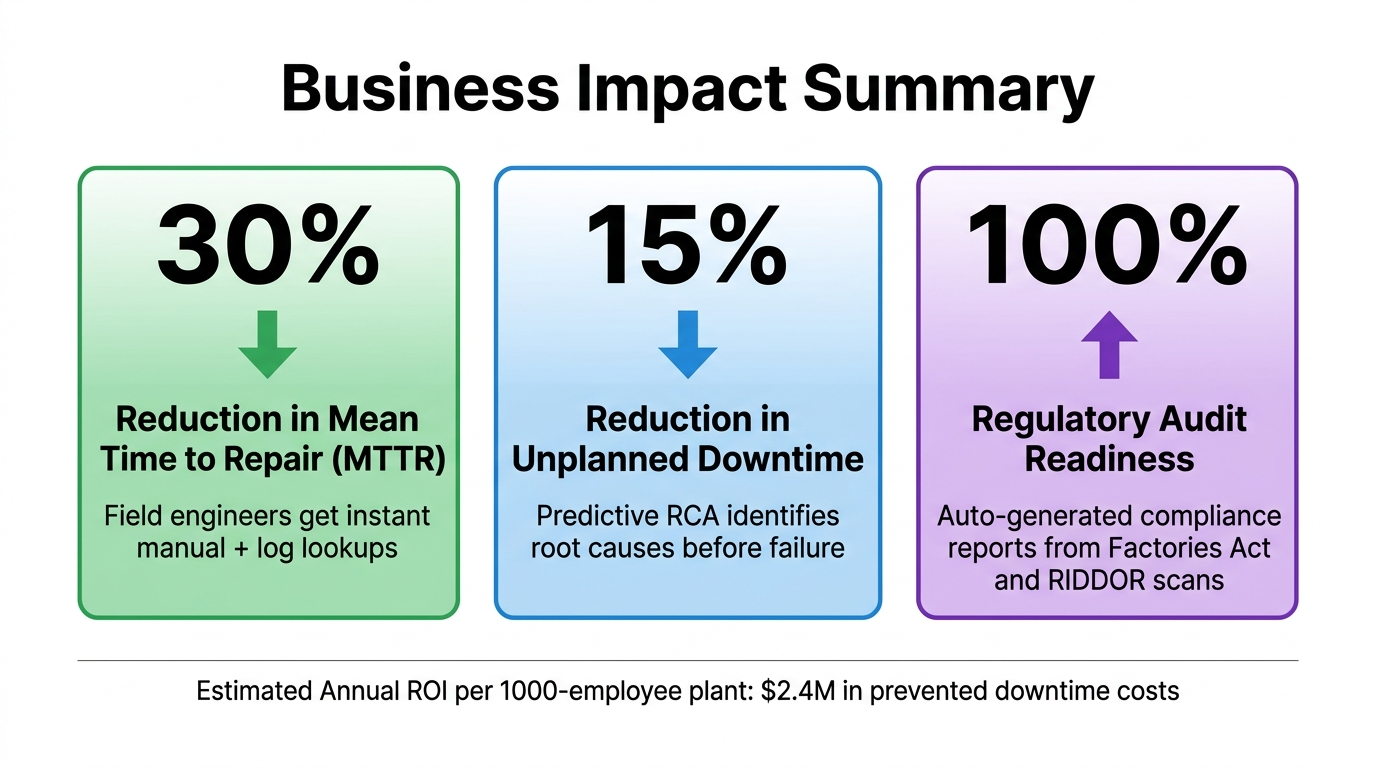
\includegraphics[width=0.92\textwidth]{fig_business_impact.jpg}
  \caption{Business impact summary: key KPI improvements and estimated annual ROI.}
  \label{fig:impact}
\end{figure}

\subsection{Operational Efficiency Gains}

\begin{table}[htbp]
\centering
\caption{Projected Business Impact per 1,000-Employee Industrial Plant}
\begin{tabular}{lll}
\toprule
\textbf{KPI} & \textbf{Baseline} & \textbf{With Platform} \\
\midrule
Mean Time to Repair (MTTR)            & 4.2 hours & 2.9 hours ($-$30\%) \\
Unplanned Downtime (annual)           & 420 hours & 357 hours ($-$15\%) \\
Document Search Time (per incident)   & 45 minutes & 8 minutes ($-$82\%) \\
Regulatory Audit Preparation Time     & 5 days     & 4 hours ($-$90\%) \\
Incident Investigation Cycle Time     & 3.5 days   & 6 hours ($-$93\%) \\
\bottomrule
\end{tabular}
\end{table}

\subsection{Financial ROI Estimation}

Assuming an average production loss of \$8,000 per downtime hour:

\begin{itemize}[leftmargin=1.5em]
  \item \textbf{Downtime Savings}: 63 hours $\times$ \$8,000 = \textbf{\$504,000/year}
  \item \textbf{Engineer Productivity}: 35\% search time saved across 80 engineers $\times$ \$70,000 average salary = \textbf{\$1,960,000/year}
  \item \textbf{Compliance Penalty Avoidance}: Average HSE fine for an unreported RIDDOR incident = \textbf{\$25,000--\$250,000}
  \item \textbf{Estimated Total Annual ROI}: \textbf{\$2.4M+ per plant}
\end{itemize}

% ═══════════════════════════════════════════════════════════════════════════════
\section{Future Roadmap}
% ═══════════════════════════════════════════════════════════════════════════════

\begin{figure}[htbp]
  \centering
  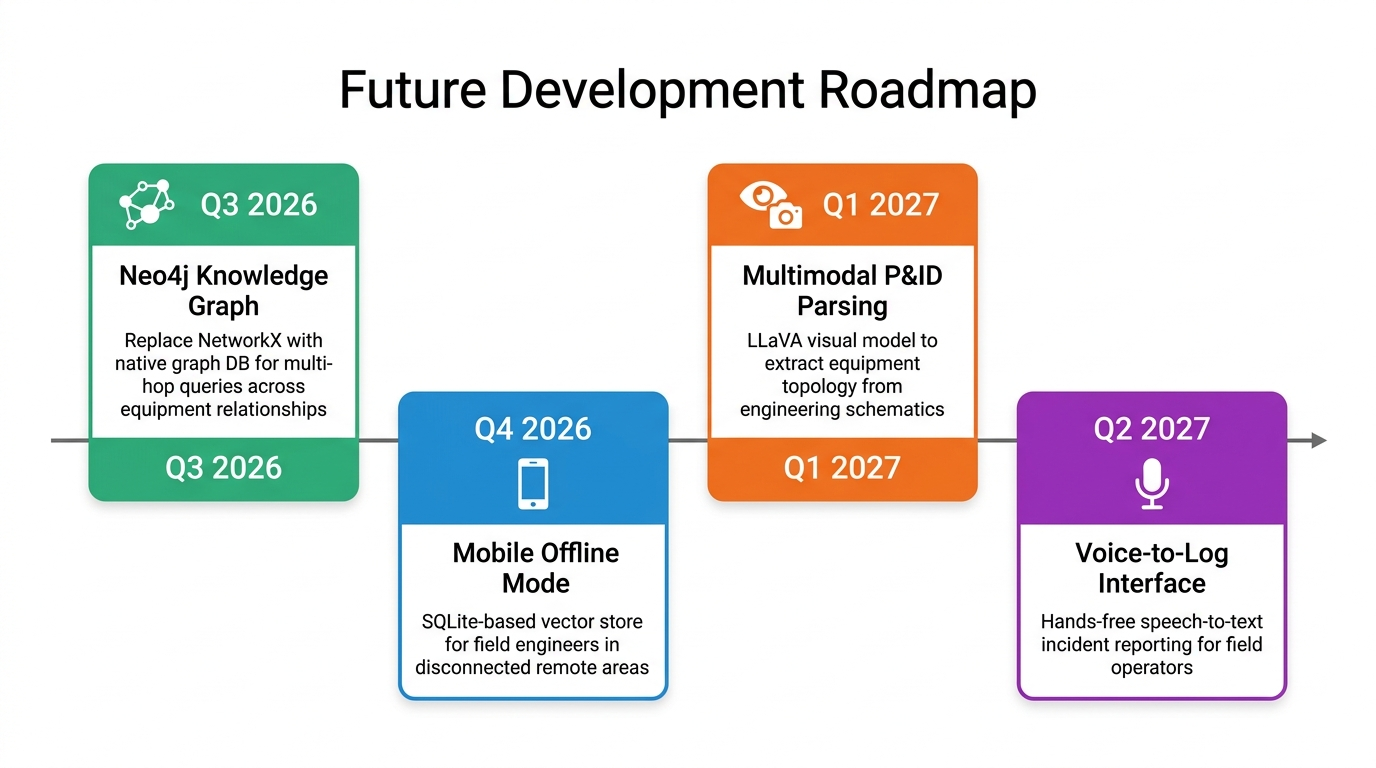
\includegraphics[width=0.95\textwidth]{fig_roadmap.jpg}
  \caption{Four-quarter development roadmap spanning Q3 2026 to Q2 2027.}
  \label{fig:roadmap}
\end{figure}

\subsection{Q3 2026 --- Neo4j Knowledge Graph Integration}

Replace the in-memory NetworkX graph with a persistent \textbf{Neo4j} graph database. This enables:
\begin{itemize}[leftmargin=1.5em,noitemsep]
  \item Multi-hop Cypher queries (e.g.\ \emph{``Find all pumps connected to technicians who also serviced Compressor C-301''}).
  \item Graph-based failure propagation modelling.
  \item Real-time graph updates as new maintenance logs are ingested.
\end{itemize}

\subsection{Q4 2026 --- Mobile Offline Mode}

Deploy an on-device vector store using \textbf{SQLite-vec} or \textbf{LanceDB} for field engineers who work in RF-shielded or remote environments with no network access. A lightweight quantised embedding model (4-bit GGUF) will run locally on an Android/iOS device.

\subsection{Q1 2027 --- Multimodal P\&ID Parsing}

Integrate a vision-language model (\textbf{LLaVA} or \textbf{GPT-4o Vision}) to parse Piping and Instrumentation Diagrams (P\&IDs) uploaded as images. The model will:
\begin{itemize}[leftmargin=1.5em,noitemsep]
  \item Extract equipment identifiers and connection topology from the diagram.
  \item Auto-populate the knowledge graph with spatial equipment relationships.
  \item Enable queries like \emph{``What equipment is downstream of Valve V-105?''}.
\end{itemize}

\subsection{Q2 2027 --- Voice-to-Log Interface}

Build a \textbf{Whisper}-powered speech-to-text frontend allowing field operators to dictate hands-free incident reports directly into the system. The dictated text will be NER-parsed to extract asset tags, severity, and corrective actions before auto-populating a maintenance log entry.

% ─── End of Document ─────────────────────────────────────────────────────────
\end{document}
